\documentclass[11pt,a4paper]{article}

\usepackage[utf8]{inputenc}
\usepackage[T1]{fontenc}
\usepackage[spanish,english]{babel}
\usepackage[a4paper,margin=2.1cm]{geometry}
\usepackage{amsmath,amssymb}
\usepackage{booktabs}
\usepackage{graphicx}
\usepackage{float}
\usepackage{hyperref}
\usepackage{enumitem}
\usepackage{xcolor}

\setlength{\parindent}{0pt}
\setlength{\parskip}{5pt}
\setlist[itemize]{leftmargin=1.4em,itemsep=2pt,topsep=2pt}

\newcommand{\slide}[1]{\newpage\section*{#1}}
\newcommand{\figpath}[1]{\texttt{\detokenize{report/figures/#1}}}
\newcommand{\say}{\textbf{Guion oral.} }
\newcommand{\content}{\textbf{Contenido de la diapositiva.} }
\newcommand{\figs}{\textbf{Gráficos / elementos visuales.} }

\begin{document}

\begin{center}
{\LARGE\bfseries Guion para exposici\'on oral -- 20 minutos\par}
\vspace{0.3cm}
{\large Statistical Characterization and Optimization of Format Changeovers in DAMM's El Prat Bottling Lines\par}
\vspace{0.2cm}
{\large Jose Calatayud Mateu\par}
\end{center}

\vspace{0.4cm}

\textbf{Estructura recomendada.} La exposici\'on debe contar una historia:
\[
\text{problema industrial}
\rightarrow
\text{datos}
\rightarrow
\text{grafo}
\rightarrow
\text{modelo estad\'istico}
\rightarrow
\text{optimizaci\'on}
\rightarrow
\text{impacto}.
\]

\begin{table}[H]\centering
\begin{tabular}{@{}clc@{}}
\toprule
Slide & Tema & Tiempo \\
\midrule
1 & T\'itulo y mensaje principal & 1 min \\
2 & Motivaci\'on industrial: OEE y changeovers & 1.5 min \\
3 & Datasets operacionales & 1.5 min \\
4 & Construcci\'on del grafo & 1.5 min \\
5 & Dataset estad\'istico y EDA & 1.5 min \\
6 & Method 1: GoF y Bayesian updating & 2 min \\
7 & Resultados Method 1 & 2 min \\
8 & Method 2: permutation tests & 2 min \\
9 & Resultados Method 2 & 1.5 min \\
10 & Metodolog\'ia de optimizaci\'on & 2 min \\
11 & GA + Optuna + grafo aprendido & 1.5 min \\
12 & Resultados de optimizaci\'on & 2 min \\
13 & Comparaci\'on visual de schedules & 1 min \\
14 & Conclusiones & 1 min \\
\bottomrule
\end{tabular}
\end{table}

% ============================================================
\slide{Slide 1 -- Title}

\content
\begin{itemize}
    \item \textbf{Statistical Characterization and Optimization of Format Changeovers in DAMM's El Prat Bottling Lines}
    \item From statistical changeover modelling to production-sequencing optimisation.
    \item Jose Calatayud Mateu.
    \item MSc in Advanced Mathematics -- Statistics.
\end{itemize}

\figs
No es necesario poner gr\'afico. Si quieres hacerlo m\'as visual, usa una imagen
de fondo industrial suave o el logo de DAMM/UAB/UB. Mant\'en esta diapositiva limpia.

\say
Good morning. In this presentation I will explain how I used one year of
operational data from DAMM's El Prat plant to model format changeovers
statistically and then use that model to optimise a weekly production schedule.

The key idea is that a changeover is not just downtime. It depends on the
sequence: producing one SKU after another can be easy or expensive depending on
brand, volume, packaging and label reference. Therefore, if we learn which
transitions are costly, we can build better production plans.

% ============================================================
\slide{Slide 2 -- Industrial Motivation: OEE And Changeovers}

\content
\[
\text{OEE} =
\underbrace{\frac{\text{run time}}{\text{planned time}}}_{\text{Availability}}
\times
\underbrace{\frac{\text{ideal cycle}\times\text{units produced}}{\text{run time}}}_{\text{Performance}}
\times
\underbrace{\frac{\text{good units}}{\text{units produced}}}_{\text{Quality}}.
\]

\begin{itemize}
    \item DAMM operates three canning lines: L14, L17 and L19.
    \item Each line produces many SKUs.
    \item SKUs differ in brand, volume, pack and label reference.
    \item Changeovers mainly affect the \textbf{Availability} term.
\end{itemize}

\figs
Pon una figura simple tipo:
\[
\text{Product A}
\longrightarrow
\boxed{\text{Changeover}}
\longrightarrow
\text{Product B}.
\]
No hace falta usar una figura externa aqu\'i. Si quieres usar imagen, puedes usar
la imagen de proceso de DAMM como contexto, pero sin cargar demasiado la slide.

\say
The industrial KPI used in the project is OEE, Overall Equipment Effectiveness.
It decomposes production losses into availability, performance and quality.

In this work, the relevant component is availability, because during a format
change the line is stopped and no saleable output is produced. This loss is
partly controllable because it depends on the sequence of products.

So the industrial question is: can we reduce avoidable downtime by choosing a
better order of SKUs?

% ============================================================
\slide{Slide 3 -- Raw Operational Datasets}

\content
\begin{table}[H]\centering
\begin{tabular}{@{}ll@{}}
\toprule
Dataset & Role \\
\midrule
\texttt{OEE} & efficiency indicators and product attributes \\
\texttt{Cambios} & observed changeover duration \\
\texttt{Tiempo} & time-accounting decomposition \\
\texttt{Volumen} & produced hL and units \\
\texttt{Mantenimiento} & maintenance contamination \\
\bottomrule
\end{tabular}
\end{table}

\[
\text{Integration key} = \text{OF, manufacturing order}.
\]

\figs
Recomendado: una versi\'on simplificada del mapa de datasets que te pas\'o DAMM,
o una red sencilla con \texttt{OF} en el centro y los cinco datasets alrededor.

\say
The data came from five operational Excel exports. They are not independent
tables; they are different views of the same manufacturing orders.

The key variable is the OF, the manufacturing order. It connects the product,
the line, the OEE record, the produced volume, the time decomposition and the
changeover information.

For the statistical model, the most important variable is
\texttt{Frecuencia Total}, from the \texttt{Cambios} file, because it gives the
observed changeover duration in hours.

% ============================================================
\slide{Slide 4 -- From Orders To A Directed Graph}

\content
\[
\text{node}
=
\text{brand}
\times
\text{volume}
\times
\text{pack}
\times
\text{label reference}.
\]

\[
\texttt{node}
=
\texttt{marca}|\texttt{volumen}|\texttt{pack}|\texttt{envase}.
\]

\[
\text{previous node } i
\longrightarrow
\text{current node } j
=
\text{directed edge } i\to j.
\]

\begin{table}[H]\centering
\begin{tabular}{@{}ll@{}}
\toprule
Edge type & Meaning \\
\midrule
\texttt{C\_brand} & brand changes \\
\texttt{C\_vol} & volume changes \\
\texttt{C\_pack} & pack changes \\
\texttt{C\_envase} & label reference changes \\
\texttt{C0\_self} & same complete node repeated \\
\bottomrule
\end{tabular}
\end{table}

\figs
Usa un dibujo de nodos y flechas. Si quieres usar una figura del proyecto,
puedes poner \figpath{problem_flow.png}, aunque esta slide tambi\'en funciona
muy bien con un esquema hecho en Canva.

\say
A changeover cannot be defined from the current order alone. It is a transition:
we need to know what was produced immediately before.

For that reason, each product configuration is converted into a graph node. The
node combines brand, volume, pack and label reference.

Then each changeover is a directed edge from the previous product node to the
current product node. The edge type is defined using a priority rule: first
brand, then volume, then pack, then label reference, and finally repeated format.

% ============================================================
\slide{Slide 5 -- Statistical Dataset And Exploratory Analysis}

\content
\begin{itemize}
    \item Post-mortem transition dataset:
    \begin{itemize}
        \item 1,986 transitions.
        \item 188 nodes.
        \item 1,358 line-specific directed edges.
    \end{itemize}
    \item Statistical duration dataset:
    \begin{itemize}
        \item 1,378 observed changeover durations.
        \item \(H_1\): 728 observations.
        \item \(H_2\): 650 observations.
        \item 184 nodes.
        \item 1,015 unique directed edges.
    \end{itemize}
\end{itemize}

\figs
Usar obligatoriamente:
\[
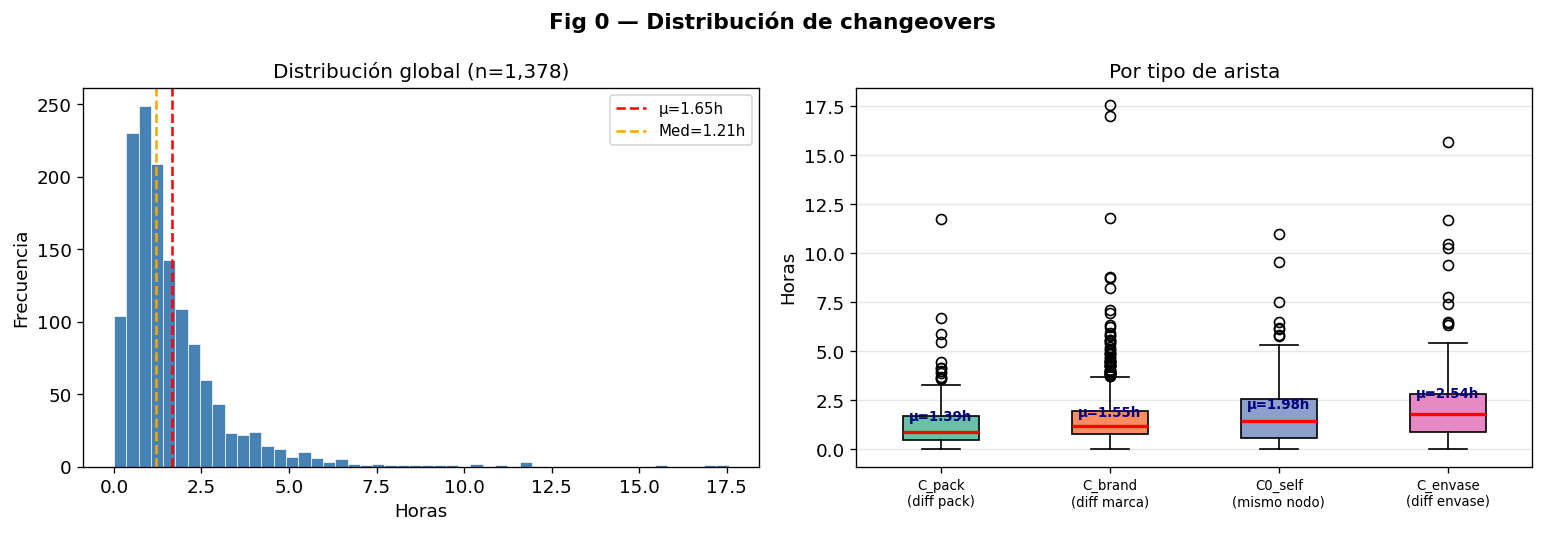
\includegraphics[width=0.88\textwidth]{report/figures/nb07_fig01.png}
\]
Archivo: \figpath{nb07_fig01.png}.

\say
There are two related datasets. The wider post-mortem dataset reconstructs all
transitions between consecutive OFs. The stricter statistical dataset only keeps
transitions with an observed duration.

The exploratory plot shows two important facts. First, durations are positive
and strongly right-skewed. Second, the sample sizes by edge type are very
unbalanced. \texttt{C\_brand} dominates, while \texttt{C\_vol} is rare.

This is why normal ANOVA or standard t-tests are not appropriate. The analysis
needs positive-skew distributions and rank-based methods.

% ============================================================
\slide{Slide 6 -- Method 1: Goodness-Of-Fit And Bayesian Updating}

\content
\[
H_1 = \text{January--June 2025},
\qquad
H_2 = \text{July--December 2025}.
\]

\[
\text{Candidate families: }
\text{Gamma},\quad
\text{Weibull},\quad
\text{LogNormal},\quad
\text{Inverse Gaussian}.
\]

\[
\text{AIC}=-2\ell(\hat{\theta})+2k.
\]

\[
D=\sup_x |F_n(x)-F(x)|,
\qquad
W^2=\int [F_n(x)-F(x)]^2\,dF(x).
\]

\figs
No pongas una figura compleja. Mejor un pipeline visual:
\[
H_1
\rightarrow
\text{fit distributions}
\rightarrow
\text{AIC + KS + CvM}
\rightarrow
\text{Bayesian cost}.
\]
Si quieres poner figura real, usa \figpath{nb07_fig02.png}, pero mejor reservar
esa para hablar de resultados.

\say
The first statistical method estimates the expected duration of a changeover.

The year is split into two halves. \(H_1\) is used to fit the initial models and
priors, while \(H_2\) is used for validation and sequential updating.

Four positive-skew families are fitted by maximum likelihood. The comparison is
based on AIC, but also on KS and Cramér--von Mises goodness-of-fit diagnostics.
The final goal is not only to describe the distribution, but to obtain a stable
cost that can be used by the optimiser.

% ============================================================
\slide{Slide 7 -- Bayesian Updating Layer}

\content
\[
X_i \mid \lambda \sim \text{Exponential}(\lambda),
\qquad
\lambda \sim \text{Gamma}(a_0,b_0).
\]

\[
p(\mathbf{x}\mid \lambda)
=
\lambda^n e^{-\lambda\sum_i x_i}.
\]

\[
\lambda \mid \mathbf{x}
\sim
\text{Gamma}
\left(
a_0+n,\;
b_0+\sum_i x_i
\right).
\]

\[
\mathbb{E}[X\mid \mathbf{x}]
=
\mathbb{E}
\left[
\frac{1}{\lambda}
\mid
\mathbf{x}
\right]
=
\frac{b_0+\sum_i x_i}{a_0+n-1}.
\]

\figs
Pon una figura conceptual de actualizaci\'on:
\[
\text{prior}
+ \text{new observations}
\rightarrow
\text{posterior cost}.
\]
No necesitas imagen externa en esta slide.

\say
The Bayesian layer uses a Gamma--Exponential conjugate model.

Here, \(\lambda\) is the rate of the exponential distribution, and \(1/\lambda\)
is the expected duration.

The advantage of this model is that the posterior has a closed form. When new
observations arrive, we only update the number of observations and the sum of
durations.

I compare two priors. The informative prior uses \(H_1\) as historical
pseudo-data. The weak prior starts almost without information and learns from
\(H_2\).

% ============================================================
\slide{Slide 8 -- Method 1 Results}

\content
\begin{table}[H]\centering
\begin{tabular}{@{}lr@{}}
\toprule
Type & Posterior mean \\
\midrule
\texttt{C\_pack} & 1.399 h \\
\texttt{C\_brand} & 1.552 h \\
\texttt{C\_vol} & 1.772 h \\
\texttt{C0\_self} & 1.995 h \\
\texttt{C\_envase} & 2.561 h \\
\bottomrule
\end{tabular}
\end{table}

\figs
Gr\'afico principal:
\[
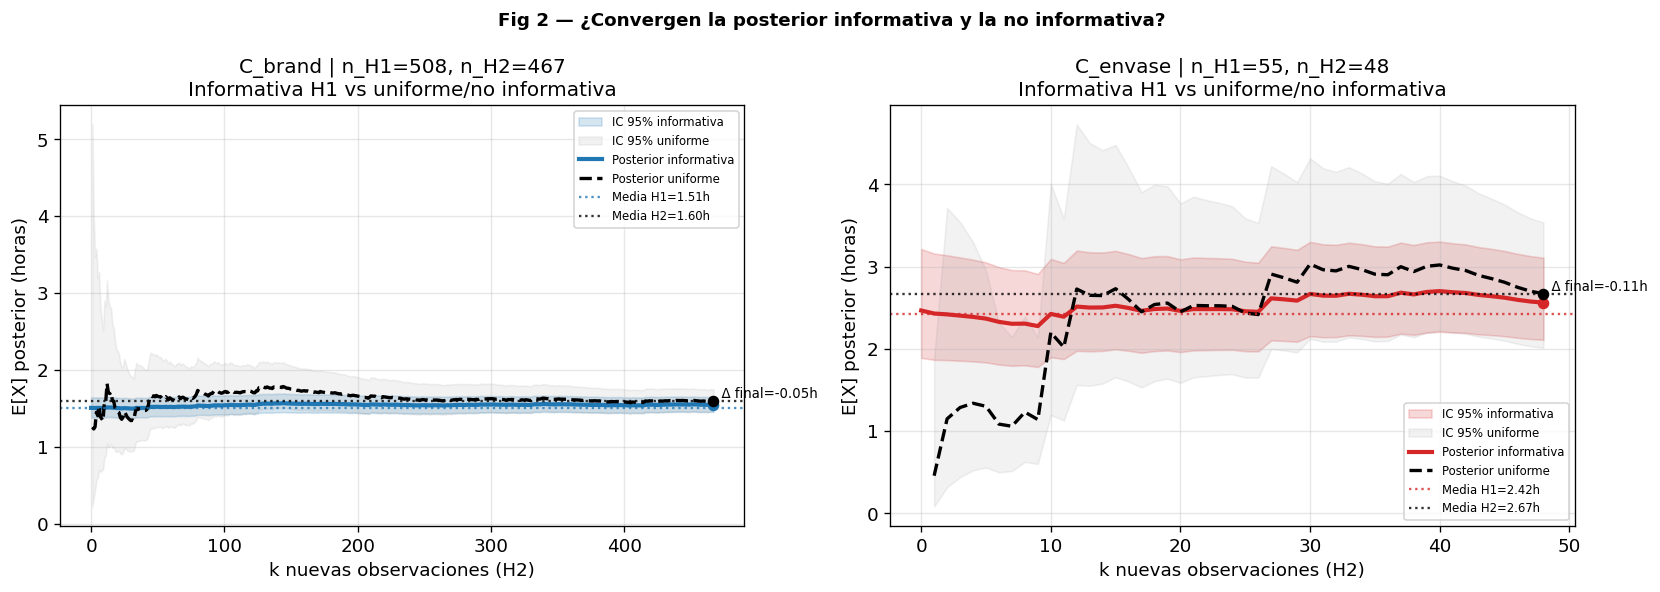
\includegraphics[width=0.88\textwidth]{report/figures/nb07_fig03.png}
\]
Archivo: \figpath{nb07_fig03.png}.

Gr\'afico opcional si tienes tiempo:
\[
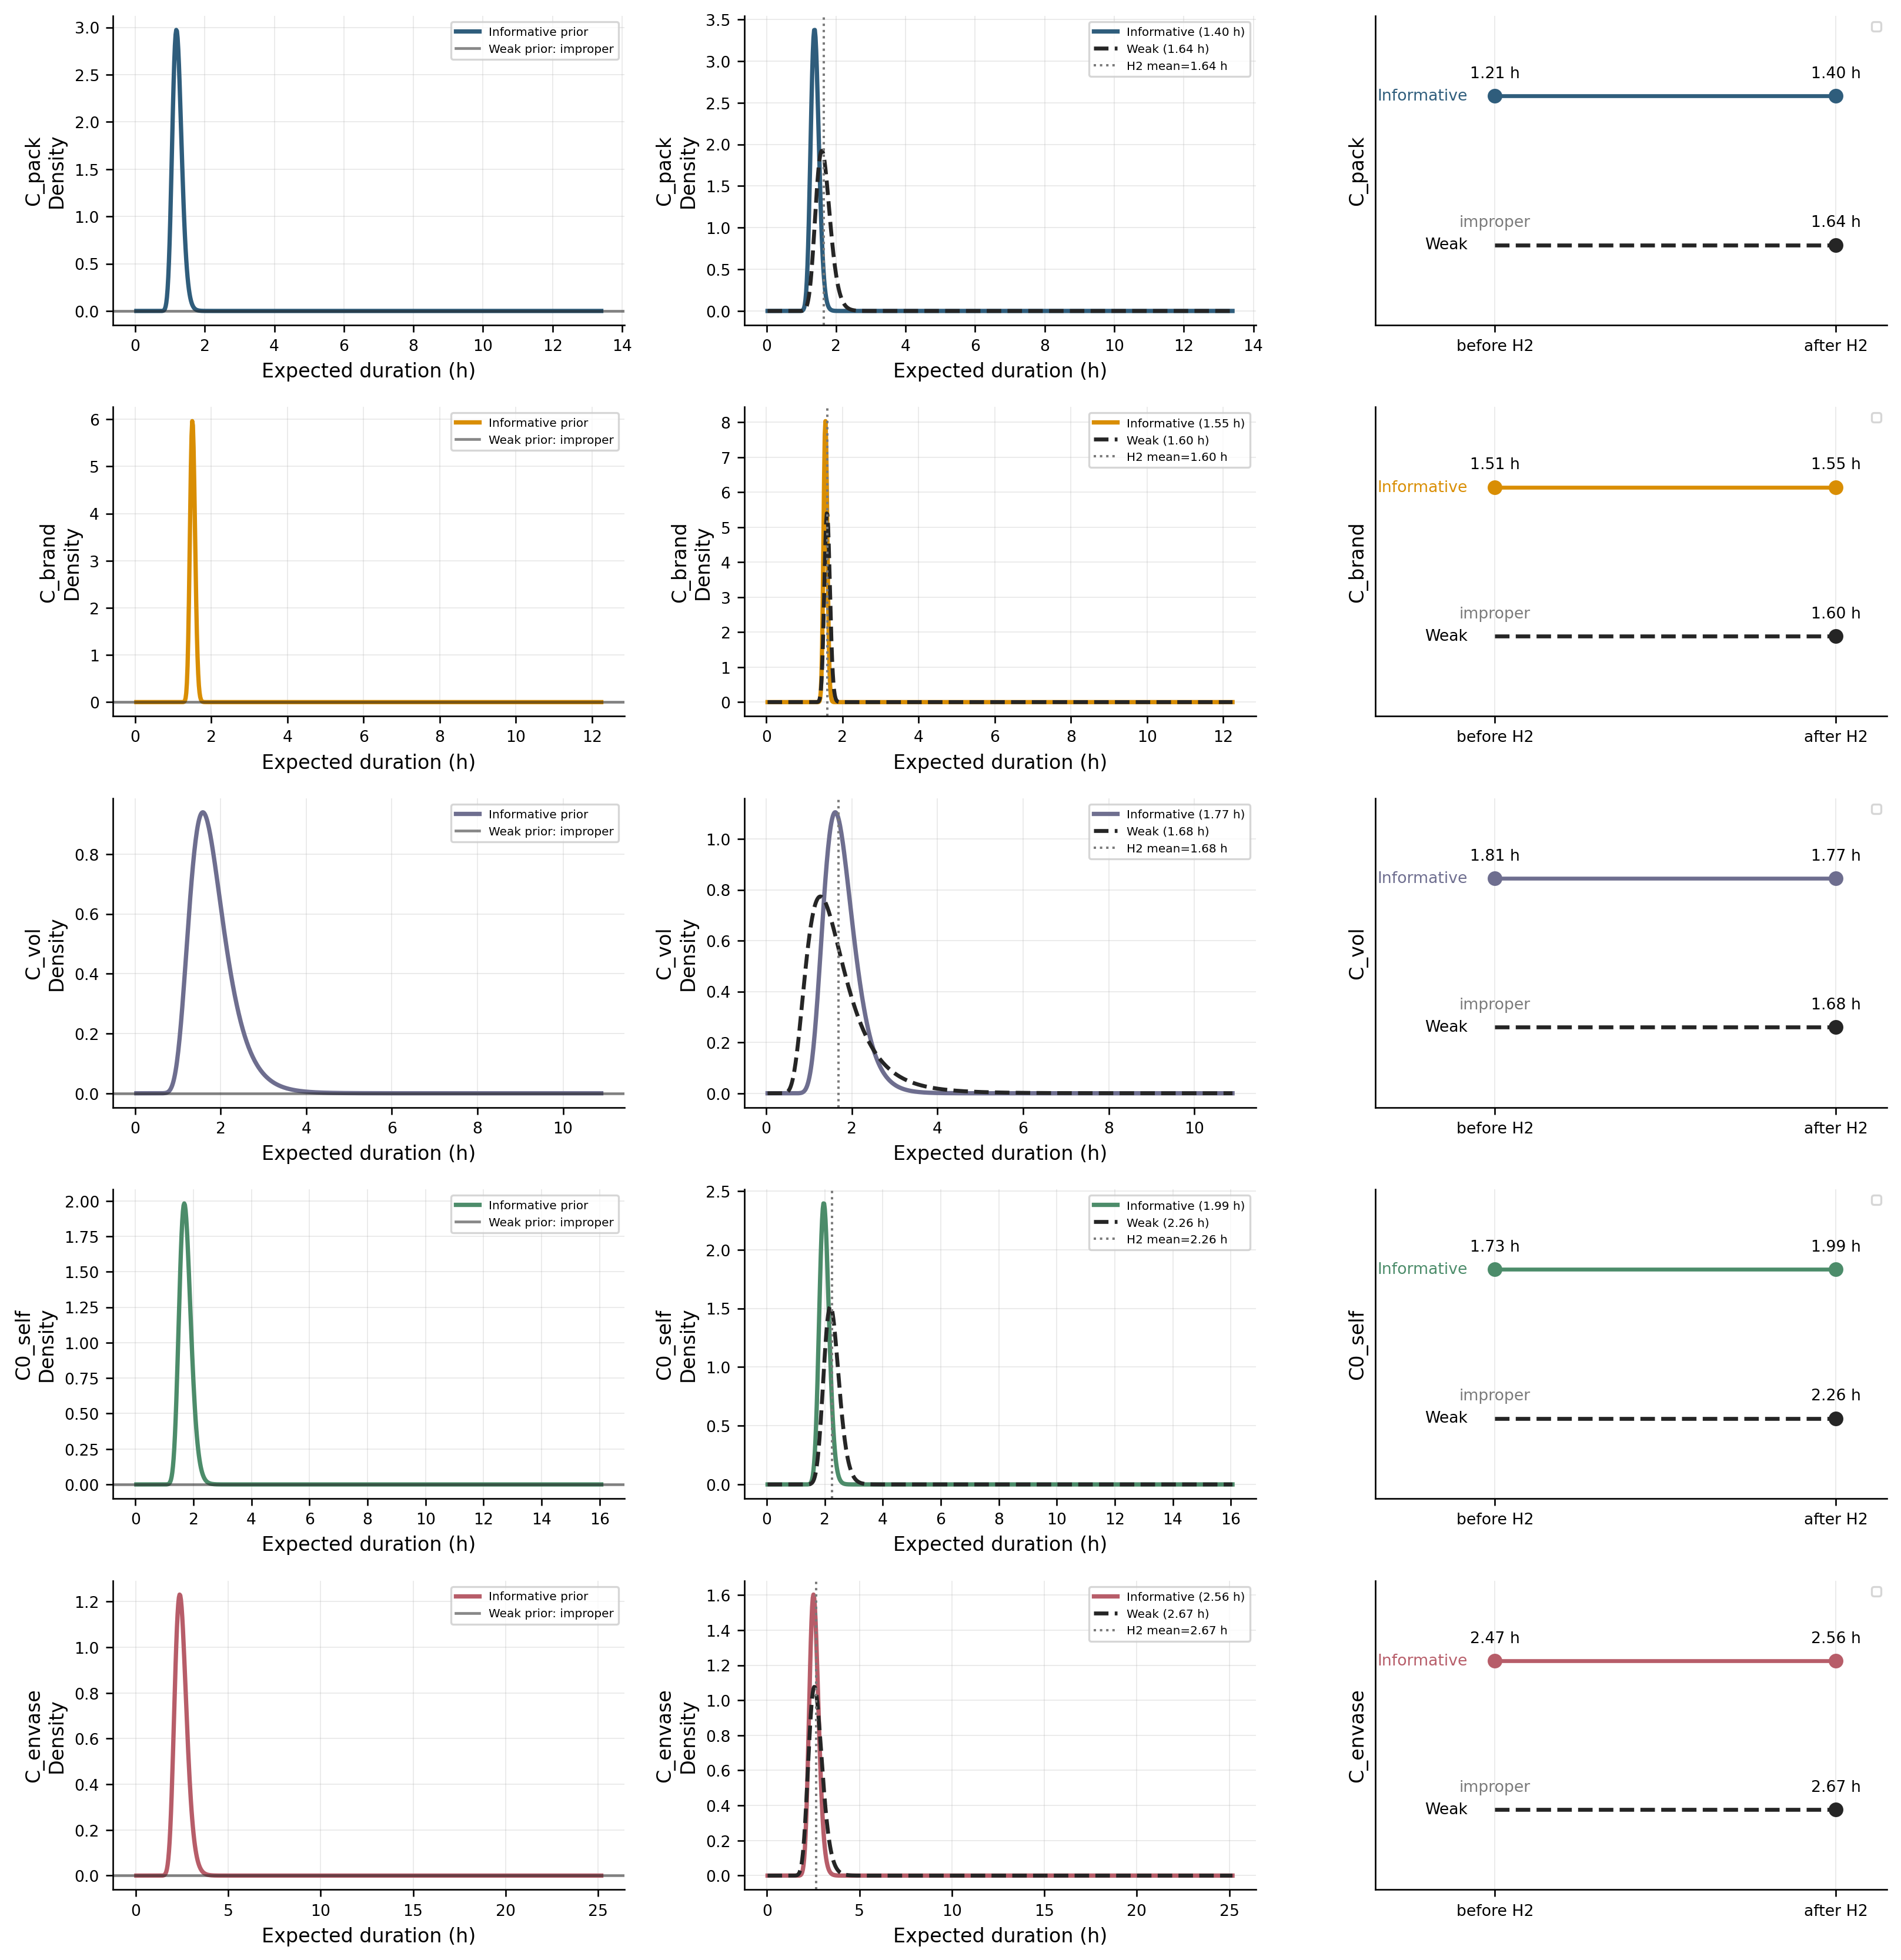
\includegraphics[width=0.72\textwidth]{report/figures/nb07_fig04.png}
\]
Archivo: \figpath{nb07_fig04.png}.

\say
The Gamma model is accepted for most edge types. For \texttt{C\_brand}, all
families are rejected because the sample is very large, so even small deviations
are detected. However, Gamma still has the lowest AIC and is kept as a fallback.

The posterior means reveal an important operational pattern:
\texttt{C\_envase}, the label-reference change, has the largest expected
duration. This is one of the main findings of the project.

The posterior plots show that informative and weak priors become close after
observing \(H_2\), meaning that the final estimate is mainly driven by the data.

% ============================================================
\slide{Slide 9 -- Method 2: Ordered Permutation Tests}

\content
\[
\texttt{C\_pack}
\leq
\texttt{C\_brand}
\leq
\texttt{C0\_self}
\leq
\texttt{C\_envase}.
\]

\[
\text{L17}
\leq
\text{L19}
\leq
\text{L14}.
\]

\[
R_i=
\frac{1}{n_i}
\sum_{j=1}^{n_i} r_{ij}.
\]

\[
T_k
=
\sum_{i<j}(R_j-R_i).
\]

\[
p=
\frac{\#\{T^{(b)}\geq T_{\text{obs}}\}+1}{B+1}.
\]

\figs
No pongas demasiadas im\'agenes aqu\'i. Esta slide es metodol\'ogica: usa las
f\'ormulas y una flecha ``rank data \(\rightarrow\) permute labels
\(\rightarrow\) p-value''.

\say
The second method tests ordered operational hypotheses.

Instead of comparing means with ANOVA, I rank all observations jointly. This is
more robust for skewed and unbalanced samples.

If the ordered alternative is true, later groups should have larger mean ranks.
The statistic \(T_k\) sums all ordered rank differences.

The p-value is obtained by permutation: under the null hypothesis, group labels
are exchangeable, so I randomly shuffle the labels 10,000 times.

% ============================================================
\slide{Slide 10 -- Method 2 Results}

\content
\[
T_4 = 863.1,
\qquad
p=10^{-4}.
\]

\[
T_3 = 285.7,
\qquad
p=10^{-4}.
\]

\begin{itemize}
    \item \texttt{C\_pack} is the lowest-cost group.
    \item \texttt{C\_envase} is the highest-cost group.
    \item L14 is significantly slower than L17 and L19.
    \item L17 and L19 are not significantly different.
\end{itemize}

\figs
Usa estos dos:
\[
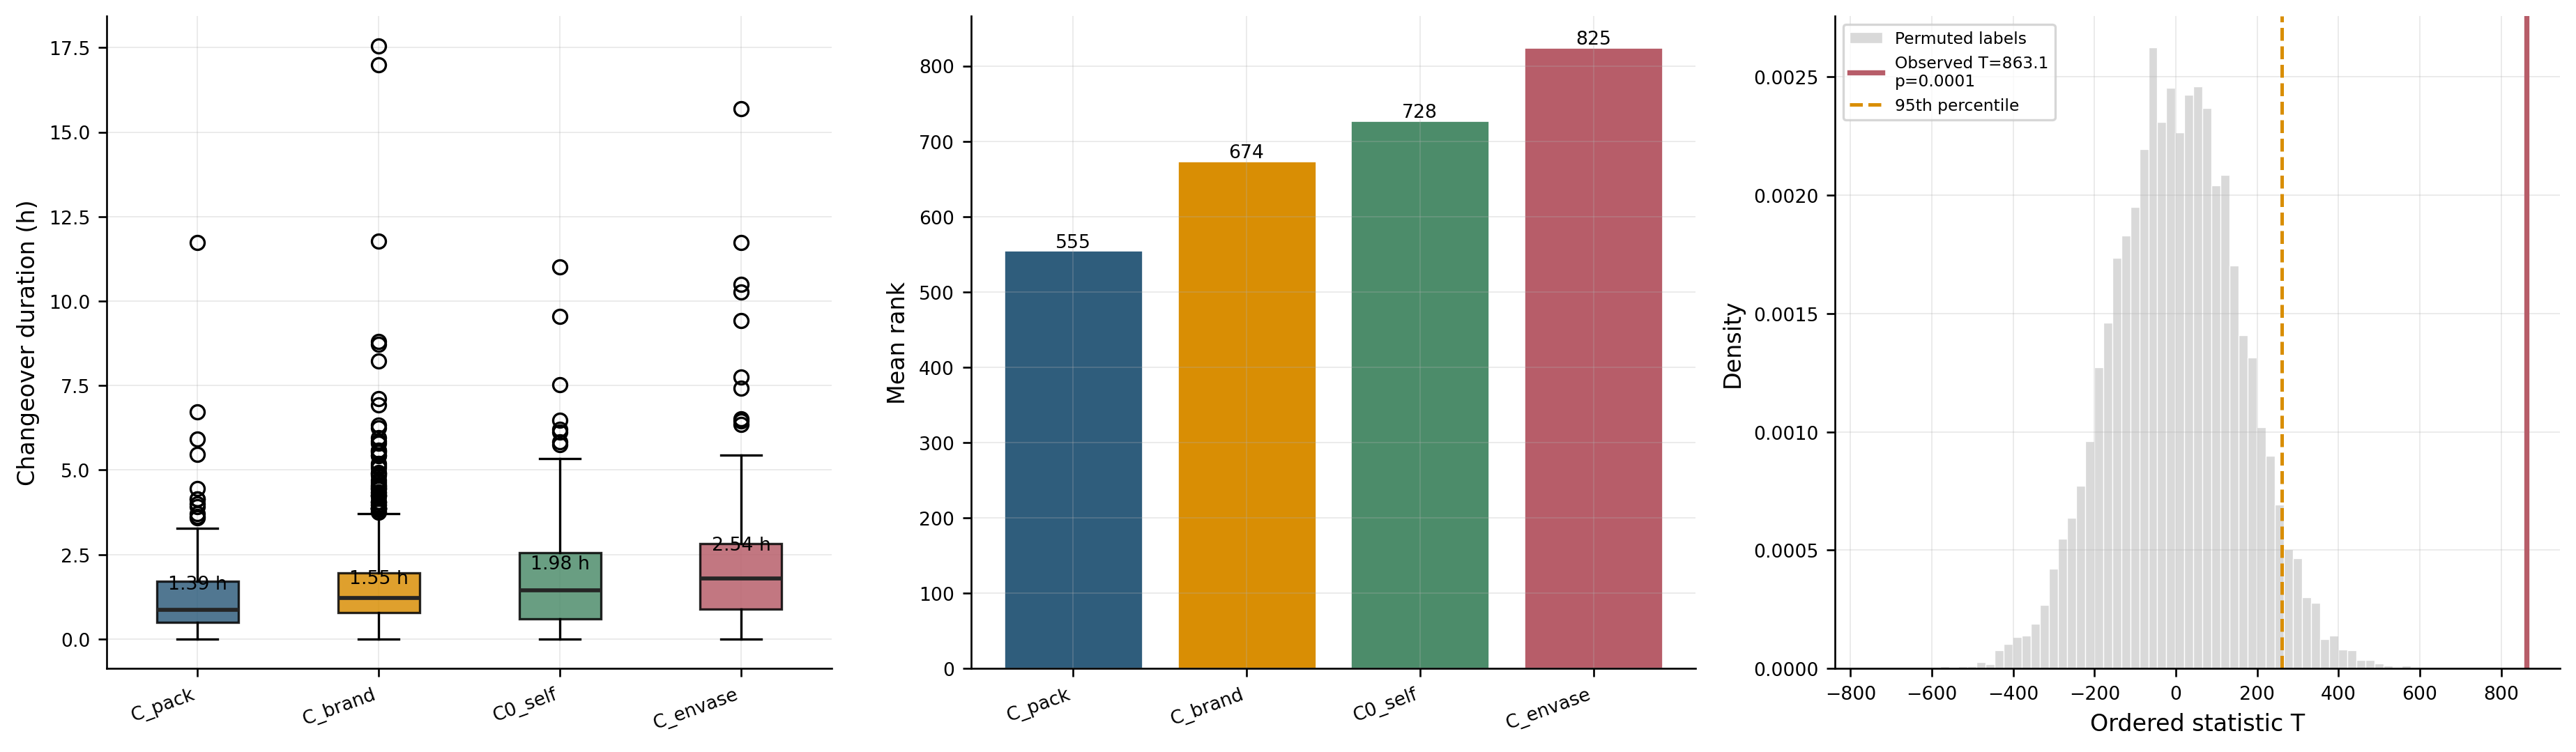
\includegraphics[width=0.82\textwidth]{report/figures/nb07_fig07.png}
\]
Archivo: \figpath{nb07_fig07.png}.

\[
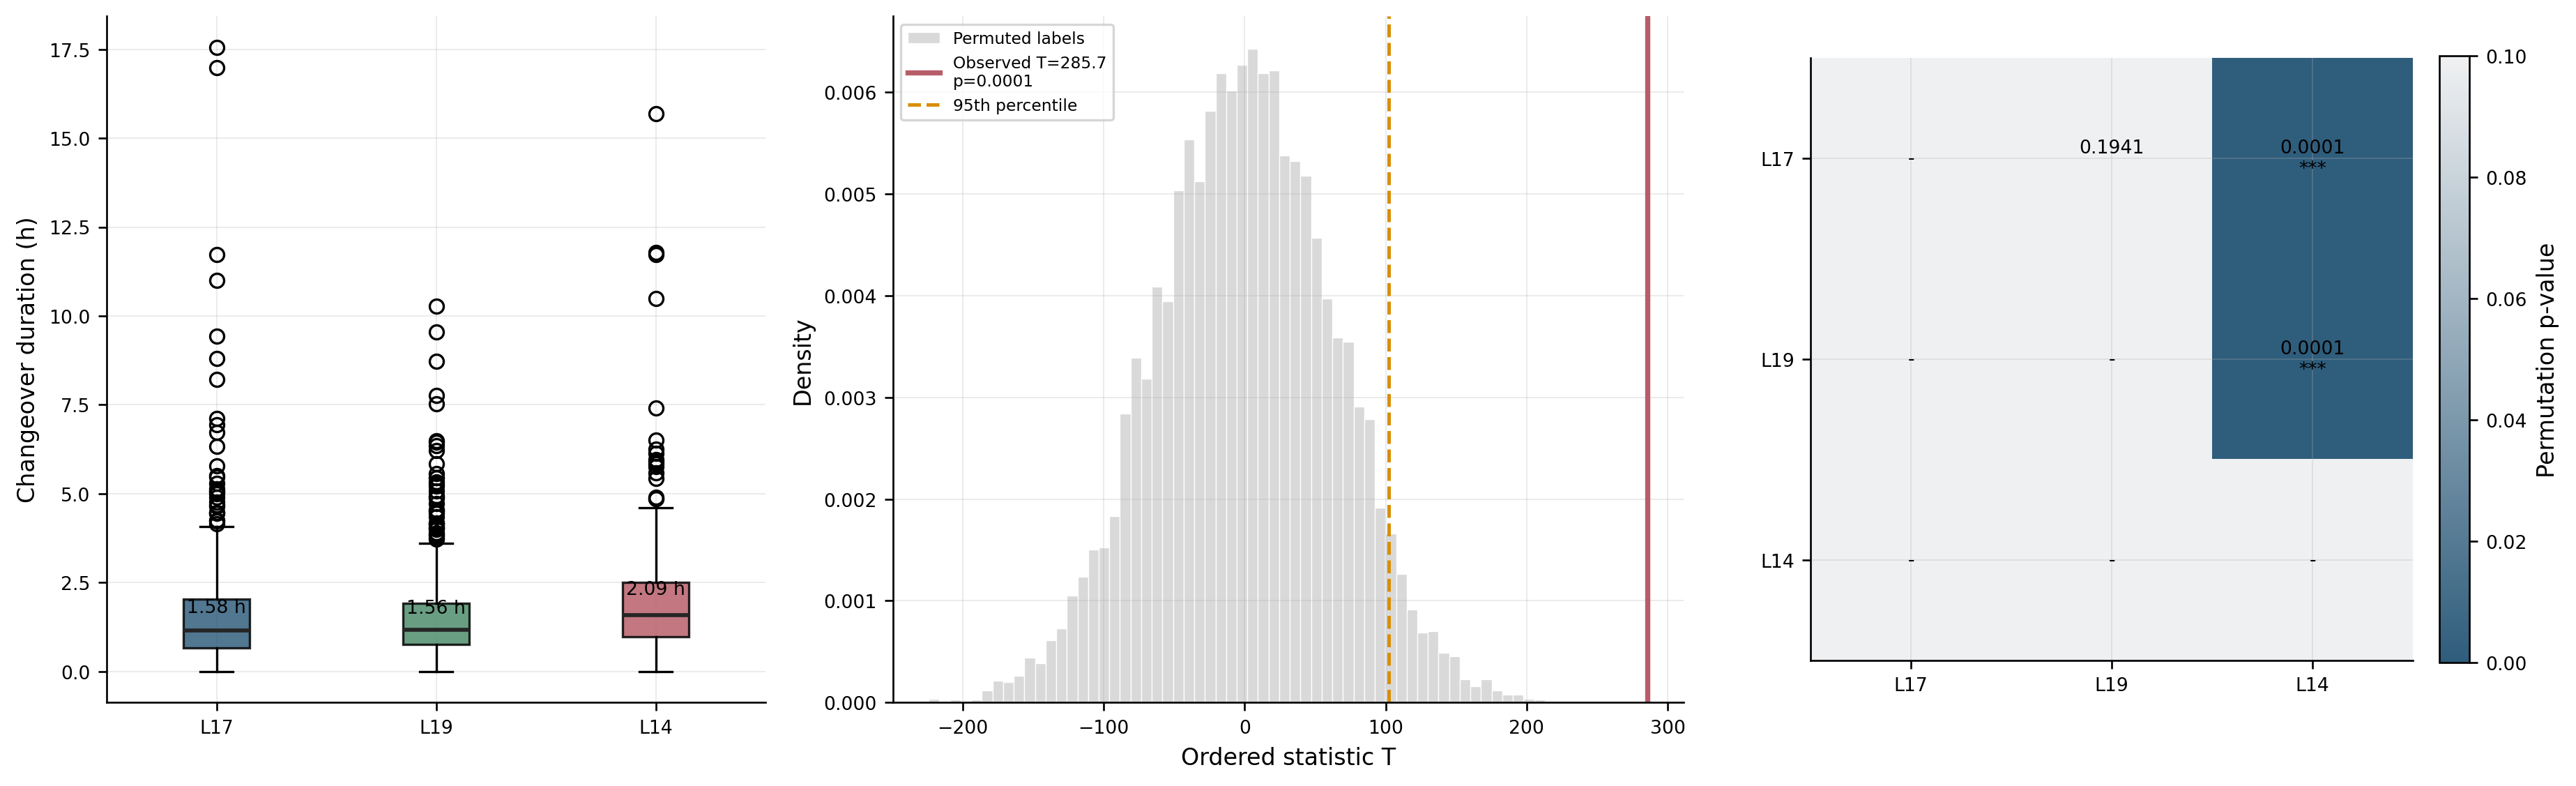
\includegraphics[width=0.82\textwidth]{report/figures/nb07_fig09.png}
\]
Archivo: \figpath{nb07_fig09.png}.

Opcional para post-hoc de edge types: \figpath{nb07_fig08.png}.

\say
The edge-type ordered test strongly rejects equality and supports the expected
difficulty pattern.

The post-hoc analysis shows that the strongest differences involve
\texttt{C\_pack} at the low end and \texttt{C\_envase} at the high end.

For lines, the ordered test also rejects equality. The post-hoc results show
that the effect is mainly caused by L14, which is significantly slower than both
L17 and L19.

% ============================================================
\slide{Slide 11 -- Optimisation Problem}

\content
\begin{itemize}
    \item Target week: 18--22 May 2026.
    \item Demand: 28 SKUs and 36,933.48 hL.
    \item Lines: L14, L17 and L19.
    \item Total weekly capacity: 340 h.
\end{itemize}

\[
H_{\ell}
=
s_{\ell}
+
\sum_{i\in S_{\ell}}
\frac{V_i}{\rho_{i\ell}}
+
\sum_{(i,j)\in A_{\ell}}
c^h_{\ell ij}.
\]

\[
\min
\sum_{\ell\in\{14,17,19\}}
H_{\ell},
\qquad
H_\ell \leq \kappa_\ell.
\]

\figs
Usa un esquema en Canva con tres cajas:
\[
\text{Demand + throughput}
\rightarrow
\text{assignment + sequencing}
\rightarrow
\text{weekly hours}.
\]
No hace falta figura externa.

\say
The optimisation problem is the weekly assignment and sequencing of the target
week.

Each SKU must be assigned to one feasible line, and the SKUs assigned to a line
must be ordered.

The total hours of a line have three components: start-up time, production time
and changeover time.

The key term is \(c^h_{\ell ij}\), the Bayesian expected changeover duration for
the transition from SKU \(i\) to SKU \(j\) on line \(\ell\).

% ============================================================
\slide{Slide 12 -- Genetic Algorithm And Optuna}

\content
\[
\{14:[\cdots],\;17:[\cdots],\;19:[\cdots]\}.
\]

\[
\text{fitness}
=
\sum_\ell H_\ell
+
P_{\text{incompatibility}}
+
P_{\text{capacity}}
+
P_{\text{urgency}}.
\]

\[
\theta_{\text{GA}}
=
(
\texttt{mut\_prob},
\texttt{elitism},
\texttt{tour\_size}
).
\]

\begin{table}[H]\centering
\begin{tabular}{@{}lr@{}}
\toprule
Hyperparameter & Value \\
\midrule
Mutation probability & 0.849 \\
Elitism & 3 \\
Tournament size & 3 \\
Best fitness & 266.45 \\
\bottomrule
\end{tabular}
\end{table}

\figs
Puedes usar una mini figura de pipeline:
\[
\text{Optuna}
\rightarrow
\text{GA hyperparameters}
\rightarrow
\text{best schedule}.
\]
Si quieres imagen real de Optuna, usa \figpath{sec06_ga_optuna_result.png}, pero
en la presentaci\'on es mejor una tabla limpia.

\say
The final optimiser is a genetic algorithm.

A schedule is represented as a chromosome with one sequence per line. Every SKU
appears exactly once across the three lists.

The fitness is total simulated hours plus penalties. The penalties ensure that
the solution respects physical compatibility, historical eligibility, capacity
and urgent orders.

Optuna is used to tune the genetic algorithm. It searches over mutation
probability, elitism and tournament size using a TPE sampler.

% ============================================================
\slide{Slide 13 -- Learned Bayesian Graph}

\content
\begin{table}[H]\centering
\begin{tabular}{@{}lr@{}}
\toprule
Quantity & Value \\
\midrule
2025 production orders & 2141 \\
Product nodes & 188 \\
Unique directed edges & 3596 \\
\bottomrule
\end{tabular}
\end{table}

\figs
Usar:
\[
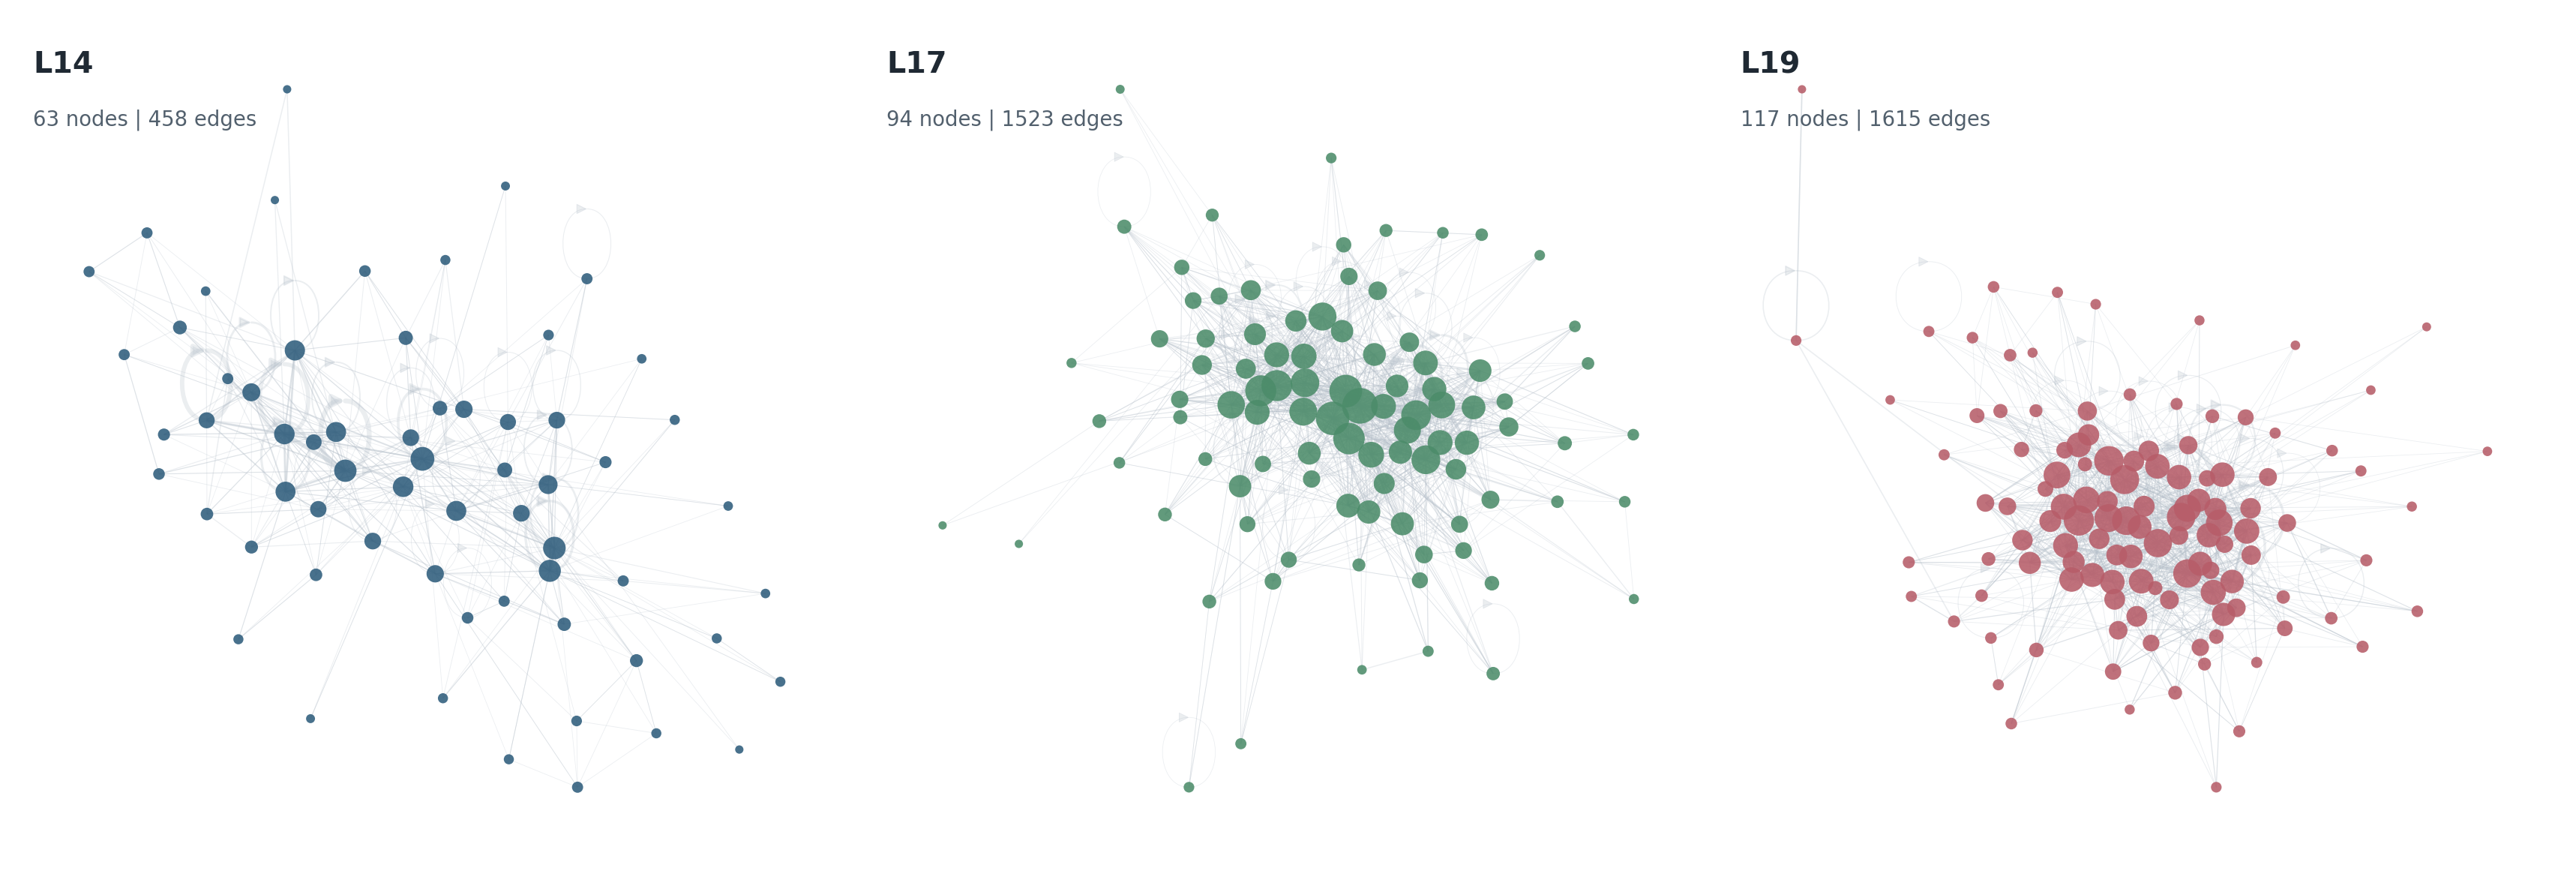
\includegraphics[width=0.9\textwidth]{report/figures/sec06_learned_graph_by_line.png}
\]
Archivo: \figpath{sec06_learned_graph_by_line.png}.

\say
The Streamlit app learns the historical Bayesian changeover graph from the 2025
production history.

The graph contains 188 product nodes and 3,596 unique directed edges.

The graph is visualised separately by line because the same product transition
can have different behaviour depending on whether it occurs on L14, L17 or L19.

This is the operational cost map used by the optimiser.

% ============================================================
\slide{Slide 14 -- Optimisation Results}

\content
\begin{table}[H]\centering
\begin{tabular}{@{}lr@{}}
\toprule
Schedule & Total hours \\
\midrule
Real executed schedule & 426.1 h \\
Theoretical planner schedule & 333.0 h \\
GA optimised schedule & 325.6 h \\
\bottomrule
\end{tabular}
\end{table}

\[
\text{Saving vs real}
=
426.1 - 325.6
=
100.6\text{ h}.
\]

\[
\text{Reduction}=23.6\%,
\qquad
59.8\%\rightarrow87.4\%,
\qquad
\Delta \text{OEE}=+27.6\text{ pp}.
\]

\figs
No pongas las tres schedules aqu\'i si tienes la siguiente slide para ello.
Aqu\'i pon una tabla limpia y un n\'umero grande:
\[
\boxed{100.6\text{ h saved}}
\]

\say
The final schedule is compared with two references: the real executed schedule
and the theoretical planner schedule.

The real schedule requires 426.1 hours. The theoretical planner requires 333.0
hours. The GA optimised schedule requires 325.6 hours.

This means a saving of 100.6 hours compared with the real executed schedule,
which is a 23.6 percent reduction.

The OEE also improves substantially, from 59.8 percent to 87.4 percent.

% ============================================================
\slide{Slide 15 -- Schedule Comparison}

\content
Mostrar las tres planificaciones en este orden:
\begin{enumerate}
    \item Theoretical planner.
    \item Real executed.
    \item GA optimised.
\end{enumerate}

\figs
Usar estas tres figuras:
\[
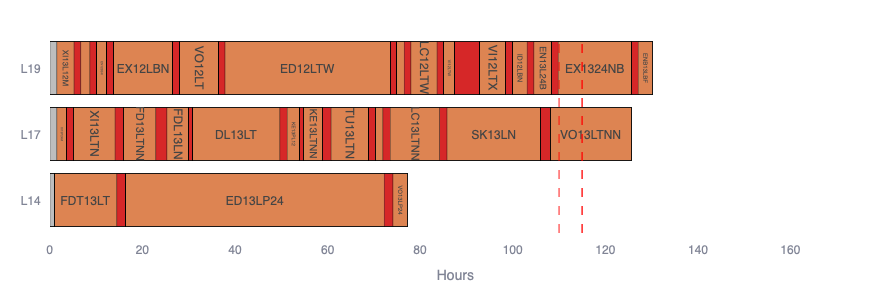
\includegraphics[width=0.88\textwidth]{report/figures/theoric_planner.png}
\]
\[
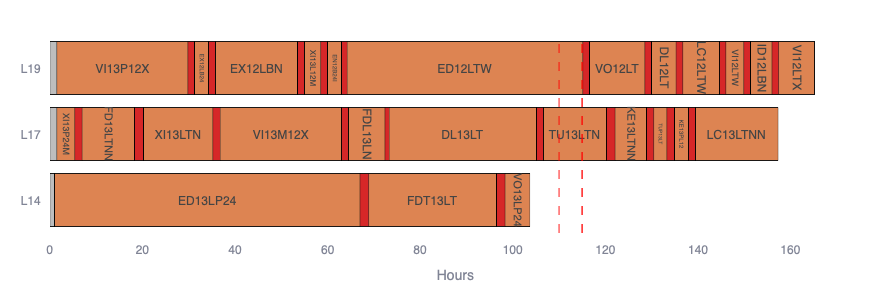
\includegraphics[width=0.88\textwidth]{report/figures/newplot-3.png}
\]
\[
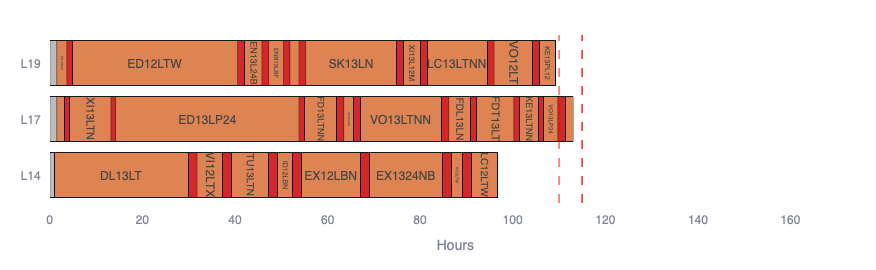
\includegraphics[width=0.88\textwidth]{report/figures/optim_planner.png}
\]

Archivos:
\begin{itemize}
    \item \figpath{theoric_planner.png}
    \item \figpath{newplot-3.png}
    \item \figpath{optim_planner.png}
\end{itemize}

\say
These three schedules show the difference visually.

The theoretical planner is already much better than the real executed schedule,
but the GA optimiser still improves it.

The optimiser changes both assignment and sequencing. Some SKUs are moved to
different lines, and the internal order of each line changes.

The purpose is not only to reduce individual changeovers, but to minimise the
total weekly execution time while keeping the plan feasible.

% ============================================================
\slide{Slide 16 -- Conclusions}

\content
\begin{itemize}
    \item Changeovers are sequence-dependent and should be modelled as graph edges.
    \item Durations are positive, skewed and unbalanced.
    \item Gamma--Exponential Bayesian updating gives an operational cost layer.
    \item Ordered rank tests show:
    \[
    \texttt{C\_pack}
    \leq
    \texttt{C\_brand}
    \leq
    \texttt{C0\_self}
    \leq
    \texttt{C\_envase}.
    \]
    \item \texttt{C\_envase} is a critical changeover type.
    \item The GA + Optuna optimiser saves 100.6 h in the target week.
\end{itemize}

\textbf{Limitations}
\begin{itemize}
    \item One year of historical data.
    \item Some directed edges are sparse.
    \item Fallback rules are needed for unseen transitions.
    \item Future work: live validation with new production weeks.
\end{itemize}

\figs
No hace falta gr\'afico. Puedes poner una frase final grande:
\[
\text{Changeovers are a statistical network problem, not only downtime.}
\]

\say
To conclude, the project connects statistical modelling and production planning.

The statistical model is not only descriptive. It becomes the cost function of
the optimiser.

The most actionable finding is that label-reference changes are expensive and
should be considered explicitly in sequencing decisions.

Finally, the optimisation results show that using learned Bayesian changeover
costs can significantly reduce weekly workload and improve OEE.

% ============================================================
\newpage
\section*{Resumen de gr\'aficos que debes poner en Canva}

\begin{table}[H]\centering\small
\begin{tabular}{@{}clp{7.2cm}@{}}
\toprule
Slide & Archivo & Uso \\
\midrule
3 & mapa DAMM o esquema propio & explicar c\'omo se conectan los datasets por OF \\
4 & \figpath{problem_flow.png} opcional & explicar nodos y edges \\
5 & \figpath{nb07_fig01.png} & EDA: distribuci\'on global y por edge type \\
8 & \figpath{nb07_fig03.png} & posterior sequential update \\
8 & \figpath{nb07_fig04.png} opcional & prior-to-posterior densities \\
10 & \figpath{nb07_fig07.png} & ordered edge-type test \\
10 & \figpath{nb07_fig08.png} opcional & post-hoc edge-type tests \\
10 & \figpath{nb07_fig09.png} & ordered line test \\
13 & \figpath{sec06_learned_graph_by_line.png} & learned Bayesian graph by line \\
15 & \figpath{theoric_planner.png} & theoretical planner schedule \\
15 & \figpath{newplot-3.png} & real executed schedule \\
15 & \figpath{optim_planner.png} & GA optimised schedule \\
\bottomrule
\end{tabular}
\end{table}

\end{document}
